\documentclass[11pt]{scrartcl}


\usepackage{fullpage}

\usepackage{listings} % Coding Syntax coloring
\usepackage{color}
\usepackage{textcomp}
\definecolor{listinggray}{gray}{0.9}
\definecolor{lbcolor}{rgb}{0.9,0.9,0.9}

\usepackage{amsmath}
\usepackage{textcomp}

\lstset{
     backgroundcolor=\color{lbcolor},
     tabsize=4,
     rulecolor=,
     language=matlab,
        basicstyle=\scriptsize,
        upquote=true,
        aboveskip={1.5\baselineskip},
        columns=fixed,
        showstringspaces=false,
        extendedchars=true,
        breaklines=true,
        prebreak = \raisebox{0ex}[0ex][0ex]{\ensuremath{\hookleftarrow}},
        frame=single,
        showtabs=false,
        showspaces=false,
        showstringspaces=false,
        identifierstyle=\ttfamily,
        keywordstyle=\color[rgb]{0,0,1},
        commentstyle=\color[rgb]{0.133,0.545,0.133},
        stringstyle=\color[rgb]{0.627,0.126,0.941},
}
\usepackage{fancyhdr,graphicx,lastpage}% http://ctan.org/pkg/{fancyhdr,graphicx,lastpage}
\fancypagestyle{plain}{
  \fancyhf{}% Clear header/footer
  \fancyhead[R]{
\includegraphics[scale=0.5]{logo.png}}% Right header
  \fancyhead[L]{\textbf{School of Electronic and Electrical Engineering}}
  %\fancyfoot[L]{Name Firstname - v1.0 \\  Date}% Left footer
  \fancyfoot[R]{\thepage\  / \pageref{LastPage}}% Right footer
}
\pagestyle{plain}% Set page style to plain.


\begin{document}
\title{ELEC2856 Assignment 1}
\subtitle{ Audio Signal Processing}
\author{Yingjie Luan}
\maketitle

\tableofcontents

\section{Introduction} % (fold)

This is the description of the computer simulation of the digital filter. Matlab code is provided as pseudo code. Overall, using professor's coefficients, a FIR filter was implemented.  

% section introduction (end)


\section{Matlab Code} % (fold)

Below is the matlab code for filter simulation:
\begin{lstlisting}[language=Matlab]
function re = note2(array)
    
    y_g = zeros(1,length(array));
    
    b_w = [-0.002693840;-0.002519748;0.005014695;
        0.015641050;0.000000000;-0.046914239;
        -0.048021820;0.083481298;0.294332820];
    temp_bw = flipud(b_w);
    b_w = [b_w;0.400000000;temp_bw];
    
    for i = 1 : (length(array)-length(b_w)+1)
        buffer = array(1,i:i+18);
        y_g(1,i) = buffer*b_w;      
    end
    
    re = y_g;
\end{lstlisting}

Below is an example of matlab code using the above code for calculating impulse response:
\begin{lstlisting}[language=Matlab]
array = zeros(1,1000);
array(500) = 1;

exp = note2(array);
\end{lstlisting}

% section matlab_code (end)

\section{Code Description} % (fold)

The code above implemented a standard FIR filter, below is an image describing its behaviour:

\begin{center}
\begin{minipage}[t]{\linewidth}

{
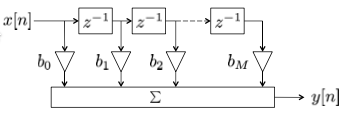
\includegraphics[scale = 1]{fir.png}
\captionof{figure}{This is description of a standard FIR filter.}
}
\end{minipage}
\medskip
\end{center}

The description goes as the following: we use an array as a length of 19 to cumulatively calculate the weighted moving average of an given array(which is going to be the input audio signal).\\


\begin{enumerate}
  \item Frequency domain description:
    $$Y(z) = (b_0 + b_1z^{-1} + b_2z^{-2} + ... +b_Mz^{-M})*X(z)$$

  \item Time domain description:
  $$y[n] = \sum^{M}_{i=0}b[i]x[n-i]$$
\end{enumerate}

And the b[i] is described both in handout and the matlab code.

An amplitude response figure is drawn given sampling rate is at 2Mhz:
\begin{center}
\begin{minipage}[t]{\linewidth}
\label{fig:test}
{
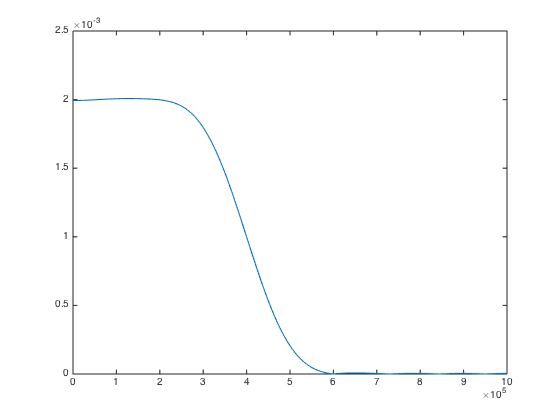
\includegraphics[scale = 0.7]{response.png}
\label{fig:tk}

\captionof{figure}{This is amplitude response. Sampling rate is supposed at 2Mhz.}
}
\end{minipage}
\medskip
\end{center}

As we can see from the figure above, the cutoff frequency is at around 0.2 of sampling rate.

% section code_descritption (end)
\end{document}


